\documentclass[xcolor=pdftex,dvipsnames,table,mathserif]{beamer}
\usetheme{default}
%\usetheme{Darmstadt}
%\usepackage{times}
%\usefonttheme{structurebold}

\usepackage[english]{babel}
%\usepackage[table]{xcolor}
\usepackage{pgf,pgfarrows,pgfnodes,pgfautomata,pgfheaps}
\usepackage{amsmath,amssymb,setspace,centernot}
\usepackage[latin1]{inputenc}
\usepackage[T1]{fontenc}
\usepackage{relsize}
\usepackage{pdfpages}
\usepackage{sgamevar}
\usepackage[absolute,overlay]{textpos} 


\newenvironment{reference}[2]{% 
  \begin{textblock*}{\textwidth}(#1,#2) 
      \footnotesize\it\bgroup\color{red!50!black}}{\egroup\end{textblock*}} 

\DeclareMathSizes{10}{10}{6}{6} 

\begin{document}
\title{Part 8: Partial Identification}
\author{Chris Conlon}
\institute{Microeconometrics}
\date{\today}

\frame{\titlepage}

\section{Intro}
\frame{\frametitle{Overview}
This Lecture will cover (roughly) the following papers:\\
Theory:
\begin{itemize}
\item Parts of Manski's book
\item Chernozhukov Hong and Tamer (2007)
\end{itemize}
Empirics:
\begin{itemize}
\item Haile and Tamer 
\end{itemize}

}

\begin{frame}
\frametitle{Motivation}
\begin{itemize}
\item Most of this course has been about what is the minimal set of assumptions we can place on our data in order to identify parameters of interest.
\item Now we consider: suppose we are willing to place even fewer assumptions on our data but are willing to accept a set of $\theta$ that satisfy our restrictions rather than a single estimate $\hat{\theta}$.
\item Reasons this might be a good idea:
\begin{itemize}
\item Maybe we don't want to impose `fully rational' behavior on agents.
\item Maybe we want to eliminate certain assumptions about functional forms, etc.
\item Maybe full solution approaches are computationally infeasible (such as complicated censoring, or dynamic games).
\end{itemize}
\end{itemize}
\end{frame}

\begin{frame}
\frametitle{Censored Data}
\begin{itemize}
\item Suppose that $Y$ is subject to censoring such that it is not always observed.
\item $(Y,X,T)$ where $T$ is a binary variable obtained by random sample.
\item $Y$ is only observed if $T=1$, $X,T$ always observed. (suppose $T=1$ is being employed).
\item In a large sample I can learn $P(X,T)$ and $P(Y | X,T=1)$ where $P(\cdot)$ is the joint distribution.
\begin{eqnarray*}
\small
P(Y| X)  = P(Y|X,T=1) P(T=1 | X) +\\
 P(Y | X,T=0) P(T=0| X)
\end{eqnarray*}
\item Challenge is that $P(Y|X,T=0)$ is unobserved and we cannot learn it without more assumptions.
\end{itemize}
\end{frame}


\begin{frame}
\frametitle{Some Ideas}
 \alert{Missing at Random}:
\begin{itemize}
\item Assume that  $Y \perp T | X$.
\begin{eqnarray*}
P(Y | X,T=1) = P(Y | X,T=0)
\end{eqnarray*}
\item $ P(Y | X,T=1) P(T=1| X) =  P(Y | X,T=0) P(T=1 | X)$ so everything is known and $P(Y|X)$ is identified.
\end{itemize}
\end{frame}


\begin{frame}
\frametitle{Suppose we know nothing...}
Then $Y \in (-\infty,+\infty)$ so the conditional expectation is unbounded!
\begin{eqnarray*}
E[Y | X] = E[Y | X, T=1] P(T=1 | X) + E[Y | X,T =0] P(T=0 | X)
\end{eqnarray*}
Now consider whether $Y \in B$ (some set). 
\begin{eqnarray*}
E[Y \in B  | X] = E[Y \in B | X, T=1] P(T=1 | X) \\
+ E[Y \in B | X,T =0] P(T=0 | X)
\end{eqnarray*}
Consider instead the probability of being in the set which is always $\in [0,1]$.
\begin{eqnarray*}
P[Y \in B  | X] = P[Y \in B | X, T=1] P(T=1 | X) \\
+ \alert{P[Y \in B | X,T =0]} P(T=0 | X)
\end{eqnarray*}
\alert{$P[Y \in B | X,T =0] $} is unknown, but it must be in $[0,1]$
\end{frame}

\begin{frame}
\frametitle{Suppose we know nothing...}
We plug in \alert{$P[Y \in B | X,T =0] =0$} and \alert{$P[Y \in B | X,T =0] =1$} :
\begin{eqnarray*}
P[Y \in B  | X]   \in ( P[Y \in B | X, T=1] P(T=1 | X),  \\
P[Y \in B | X,T =1] P(T=1 | X) + P(T=0|X)  )
\end{eqnarray*}
\begin{itemize}
\item The width of the interval is $P(T=0| X)$ so the more data are missing, the less we know.
\item We say that $P(Y \in B | X)$ is \alert{partially identified}.
\item This is the best we can do without further information \alert{bounds are sharp}.
\end{itemize}
\end{frame}


\begin{frame}
\frametitle{Add an Exclusion Restriction}
\begin{itemize}
\item Break up $X$ into $(W,V)$ so that $P(Y | W,V) = P(Y | W)$ (it does not depend on $V$).
\item This is like having $V$ be an instrumental variable.
\item Assume $V$ takes on $v_1,v_2$ to make algebra easy.
\item Now we have two restrictions:
\end{itemize}
\begin{eqnarray*}
P(Y \in B | W,V=v_1, T=1) P(T=1 | W, V=v_1) \leq  \alert{P(Y \in B | W)} \\
P(Y \in B | W,V=v_2, T=1) P(T=1 | W, V=v_2) \leq  \alert{P(Y \in B | W)} \\
\alert{P(Y \in B | W)} \leq P(Y \in B | W,V=v_1, T=1) P(T=1 | W, V=v_1) \\
+ P(T=0 | W,V=V_1)  \\
\alert{P(Y \in B | W)} \leq P(Y \in B | W,V=v_2, T=1) P(T=1 | W, V=v_2) \\
+ P(T=0 | W,V=V_2)  \\
\end{eqnarray*}
\end{frame}


\begin{frame}
\frametitle{Add an Exclusion Restriction}
Construct the \alert{greatest lower bound}:
\begin{eqnarray*}
\max_j P(Y \in B | W,V=v_j, T=1) P(T=1 | W, V=v_j) 
\end{eqnarray*}
Construct the \alert{least upper bound}:
\begin{eqnarray*}
\min_j P(Y \in B | W,V=v_j, T=1) P(T=1 | W, V=v_j) \\
 + P(T=0|W,V=v_j)
\end{eqnarray*}
With a number of levels of the instrument this can reduce the width of the interval substantially.
\end{frame}

\begin{frame}
\frametitle{Treatment Effects}
\begin{itemize}
\item Recall for treatment effects we observed $Y(1)$ only for individuals for whom $T=1$ and $Y(0)$ only for individuals for whom $T=0$.
\item $Y = Y(1) * T + Y(0) * (1-T)$.
\item We can learn $P(X,T)$ and $P(T | X)$ as well as $P(Y(1) | X,T=1)$ and $P(Y(0) | X,T=0)$.
\item We do not learn the counterfactuals: $P(Y(1) | X,T=0)$ and $P(Y(0) | X,T=1)$.
\item We are interested in $ATE(X) = E[Y(1) | X] - E[Y(0) | X]$.
Write the following:
\begin{eqnarray*}
E[Y(1) | X] = E[Y(1) | X,T=1] P(T=1 | X)  +\\
 \alert{E[Y(1) | X,T=0]} P(T=0 | X)
\end{eqnarray*}
Can we put restrictions on $ E[Y(1) | X,T=0]$ other than $(-\infty,\infty)$?
\end{itemize}
\end{frame}

\begin{frame}
\frametitle{Binary Outcomes}
\begin{itemize}
\item If $Y(1),Y(0)$ are binary outcomes then $E[Y(1) | X,T=0] \in[0,1]$ and $E[Y(0) | X,T=1] \in[0,1]$. 
\item Upper Bound on $ATE(X)$
\begin{eqnarray*}
E[Y(1) | X,T=1] P(T=1 | X) &+& P(T=0 | X)  \\
-E[Y(0) | X,T=0] P(T=0 |X) &&
\end{eqnarray*}
\item Lower Bound on $ATE(X)$
\begin{eqnarray*}
E[Y(1) | X,T=1] P(T=1 | X) &-& P(T=1 | X)  \\
-E[Y(0) | X,T=0] P(T=0 |X) &&
\end{eqnarray*}
\item So width is $P(T=0 | X) + P(T=1 |X)$.
\item We can also allow $P(Y(1) \in B |X ) - P(Y(0) \in B|X)$ using the same argument.
\end{itemize}
\end{frame}


\begin{frame}
\frametitle{More Assumptions/Tighter Bounds}
By making additional assumptions we can improve the bounds:
\begin{itemize}
\item Unconfounded treatment assignment: $T \perp Y(1),Y(0) | X$.
\begin{itemize}
\item $E[Y(1) | X, T=1] = E[Y(1) | X,T=0]$ and $E[Y(0) | X, T=1] = E[Y(0) | X,T=0]$
\item  Leads to point identification of $ATE(x)$ even if $Y$ unbounded.
\end{itemize}
\item Ordered outcomes: $Y(1) \geq Y(0)$ for all individuals
\item Roy Model: Individuals choose $T$ leading to highest outcome
\begin{itemize}
\item $Y(1) > Y(0) \rightarrow T=1$
\item $Y(1) \leq Y(0) \rightarrow T=0$
\end{itemize}
\end{itemize}
\end{frame}


\begin{frame}
\frametitle{The Mixing Problem}
\begin{itemize}
\item Drop $X$ to make life easy.
\item Recall that a randomized experiment identifies both $P(Y(0))$ and $P(Y(1))$. In large samples we can learn about the \alert{marginal distributions} of $Y(0)$ and $Y(1)$.
\item The randomized experiment tells us what happens if everyone gets $T=0$ or everyone gets $T=1$.
\item Often we are interested in something else.
\item Program is available to everyone but voluntary.
\item We make treatment available only to some people, and doctors/caseworkers decide whether to give the treatment.
\item This is known as the \alert{mixing problem}.
\end{itemize}
\end{frame}

%\begin{frame}
%\frametitle{The Mixing Problem}
%\begin{eqnarray*}
%\end{eqnarray*
%\end{frame}




\section{Partial Identification}
\frame{\frametitle{Haile and Tamer (2003)}
\begin{block}{Ascending (English) Auctions}
\begin{itemize}
\item Often modeled as button auction. 
\item Good for theory, not as good empirically.
\item Jump bidding, non-bidding, not bidding your value, etc.
\item Haile and Tamer investigate a bounds approach, which is elegant and likely to have application in other assymetric information problems.
\end{itemize}
\end{block}
\begin{exampleblock}{Assumptions}
\begin{itemize}
\item A1: Bidders do not bid above their valuation $b_{it} \leq u_{it}$ $\forall i$.
\item A2: Bidders do not let someone else win at a price they are willing to beat. 
\end{itemize}
Note: this allows for jump bidding, bids $\neq$ valuations, etc.
\end{exampleblock}
}
\frame{\frametitle{Haile and Tamer (2003)}
\footnotesize
The assumptions imply that $b^{(i;n)} \leq u^{(i;n)}$
\begin{eqnarray*}
G_B^{(i;n)}(u) \geq F_U^{(i;n)} (u) \quad \forall i,u,n
\end{eqnarray*}
We use the properties of order statistics for an iid sample of size $n$ from distribution $F$.
\begin{eqnarray*}
F_{(i:n)} (s) = \frac{n!}{(n-i)! (i-1)!} \int_{0}^{F(s)} t^{i-1}(1-t)^{n-1} dt
\end{eqnarray*}
This is increasing in $F(\cdot) \in [0,1]$ so that $F^{(i:n)}(s)$ uniquely determines values for $F(s) \forall s$.\\

Then we can define an implicit mapping where $\phi : F^{(i:n)} \rightarrow F(s)$
\begin{eqnarray*}
H &=& \frac{n!}{(n-i)! (i-1)!} \int_{0}^{\phi} t^{i-1}(1-t)^{n-1} dt \quad H \in [0,1]\\
F_U(u) &=& \phi  (F_U^{i:n}(u); i,n) 
\end{eqnarray*}
}

\frame{\frametitle{Haile and Tamer (2003)}
\footnotesize
\begin{exampleblock}{Upper Bound}
Since $\phi: [0,1] \rightarrow [0,1]$ is strictly increasing then:
\begin{eqnarray*}
\phi(G_B^{i:n}(u); i,n) \geq F_U(u)
\end{eqnarray*}
So given an estimate of $G_B^{i:n}(u)$ we can get an upper bound on $F_U(x)$. The most informative (least) upper bound is
\begin{eqnarray*}
F_U^{+}(u) = \min_{i,n} \phi(G_B^{i:n}(u);i,n)
\end{eqnarray*}
\end{exampleblock}
\begin{exampleblock}{Lower Bound}
[A2] tells us that losing bidders have valuations less than $b^{n:n} + \Delta$, where $\Delta$ is the min bid increment.
\begin{eqnarray*}
u^{n-1:n} < b^{n:n} + \Delta\\
G_{\Delta}^{n:n} (u) \leq F_U^{n-1:n}(u) \quad \forall n,u
\end{eqnarray*}
Look for greatest of $| \{\underline{n},\ldots,\overline{n}\} | $ lower bounds.
\end{exampleblock}
}

\frame{\frametitle{Haile and Tamer (2003)}
\footnotesize
\begin{exampleblock}{Nonparametric Estimator}
Easy to construct non-parametric estimators
\begin{eqnarray*}
\hat{G}_B^{i:n}(b) &=& \frac{1}{T_n} \sum_{t=1}^T \mathbb{I}[n_t =n, b^{i:n_t} \leq b]\\
\hat{G}_B^{n:n}(b) &=& \frac{1}{T_n} \sum_{t=1}^T \mathbb{I}[n_t =n, b^{n:n_t} + \Delta_t \leq b]\\
\end{eqnarray*}
\end{exampleblock}
Plug in to get bounds.  Trick is in asymptotics (bootstrap goes through).
\begin{alertblock}{Potential Problem}
In finite sample bounds may cross $\rightarrow$ work with weighted averages.
\end{alertblock}
}

\frame{\frametitle{Haile and Tamer (2003)}
\centering
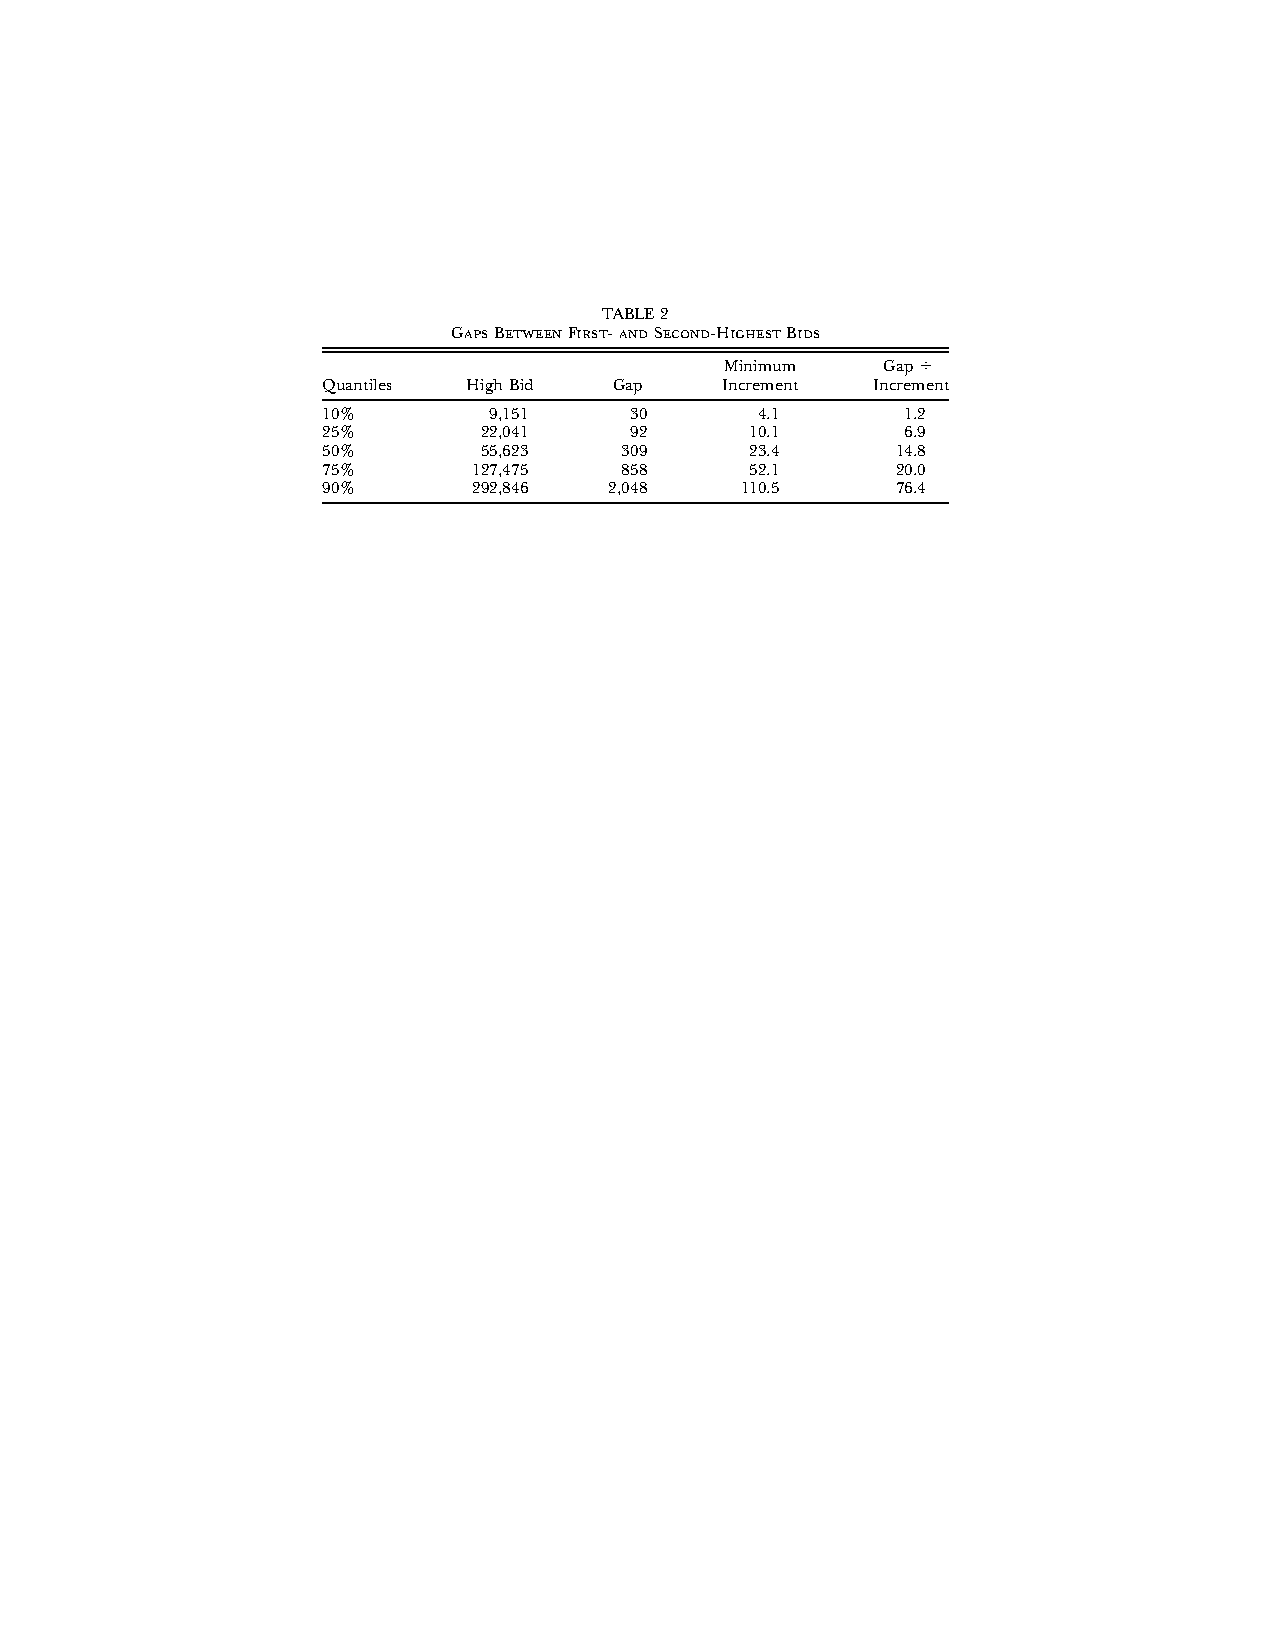
\includegraphics{./resources/hailetamer1.pdf}
}

\frame{\frametitle{Haile and Tamer (2003)}
\centering
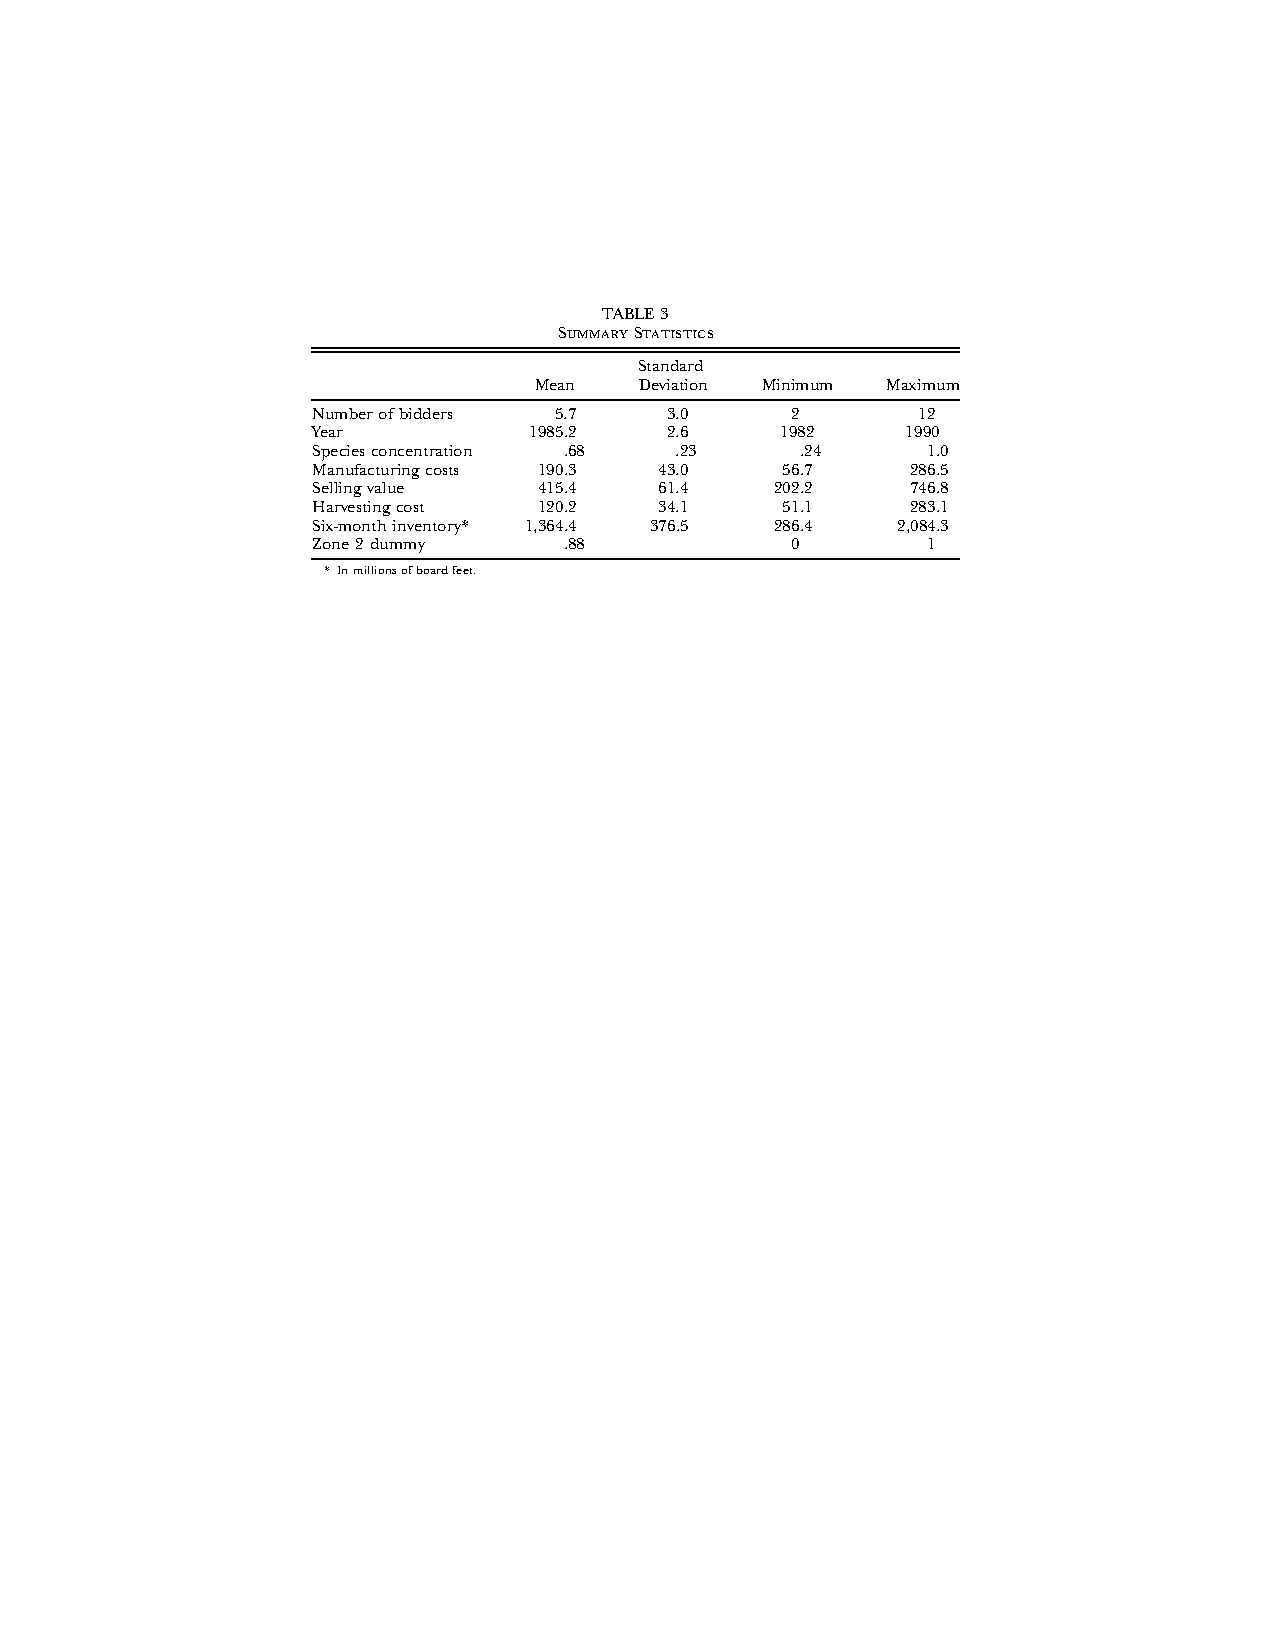
\includegraphics{./resources/hailetamer2.pdf}
}

\frame{\frametitle{Haile and Tamer (2003)}
\centering
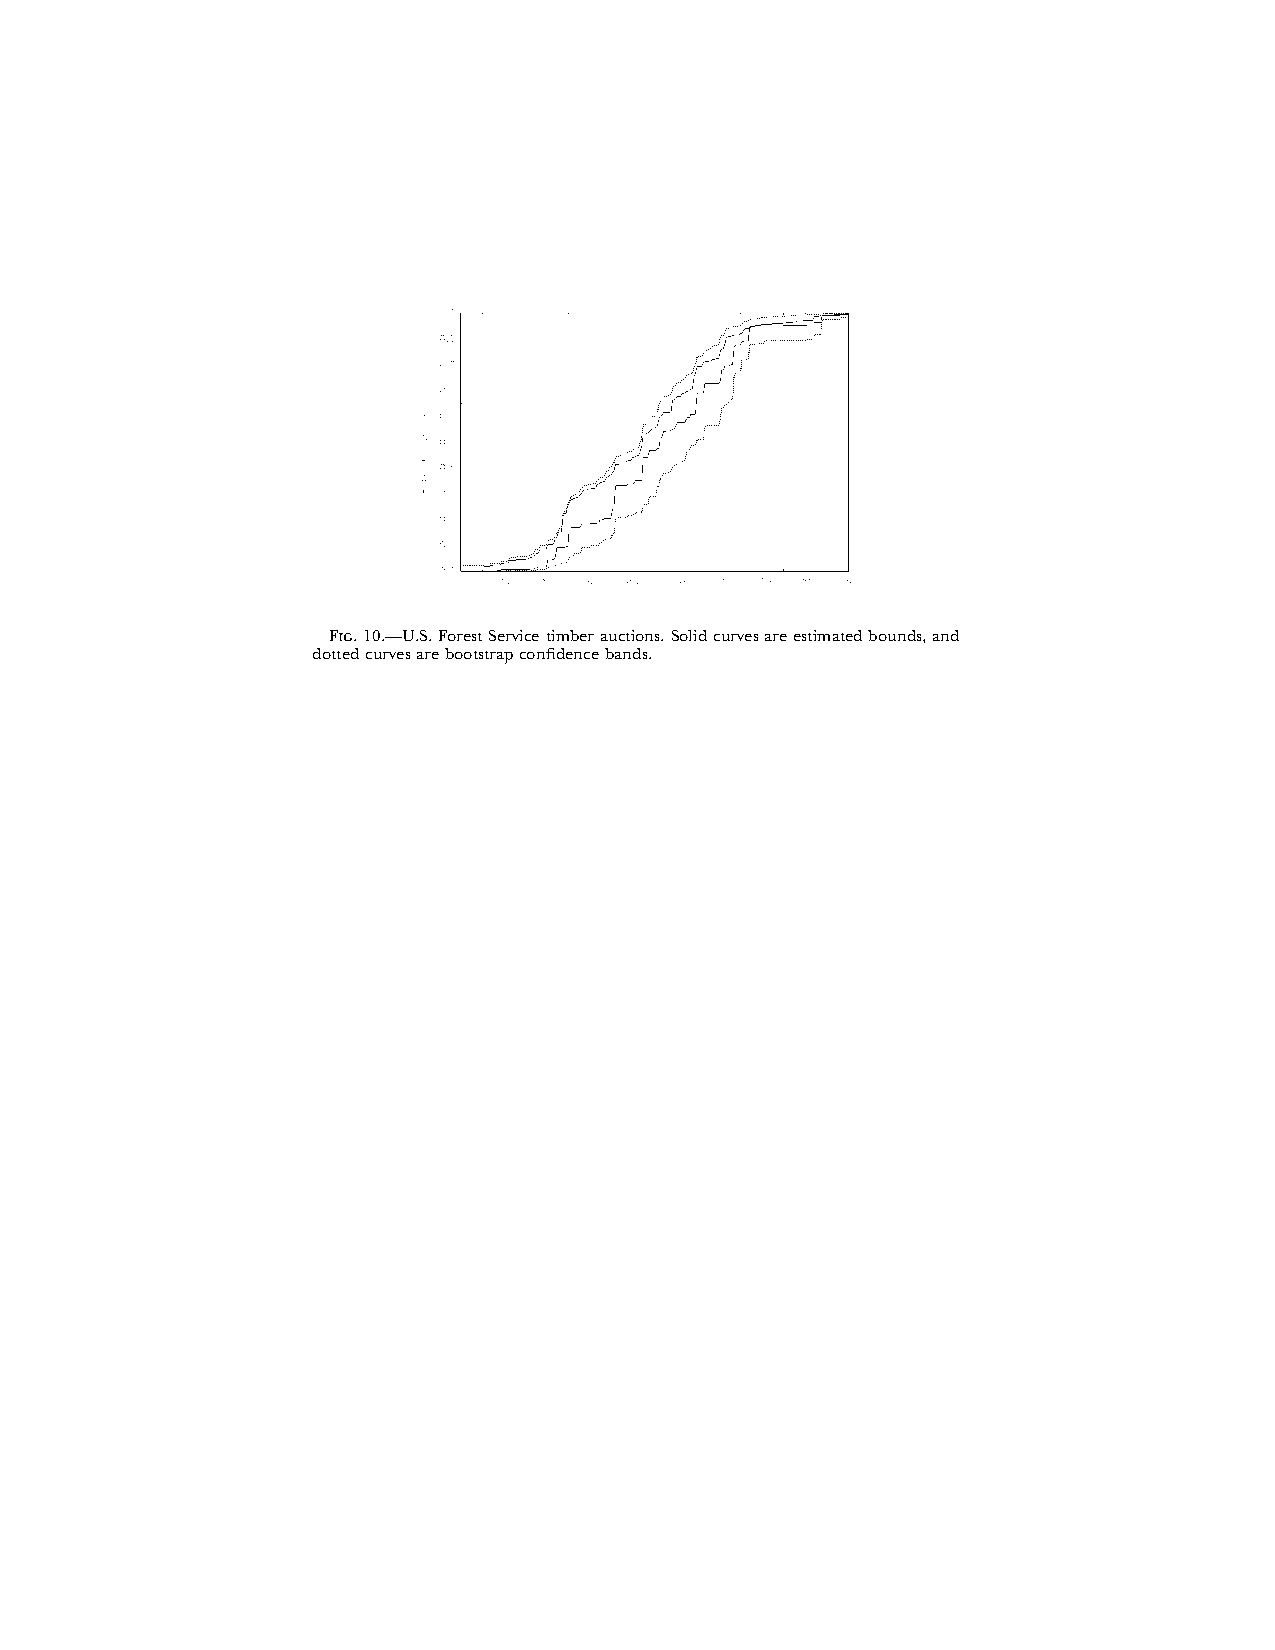
\includegraphics{./resources/hailetamer3.pdf}
}

\frame{\frametitle{Haile and Tamer (2003)}
\centering
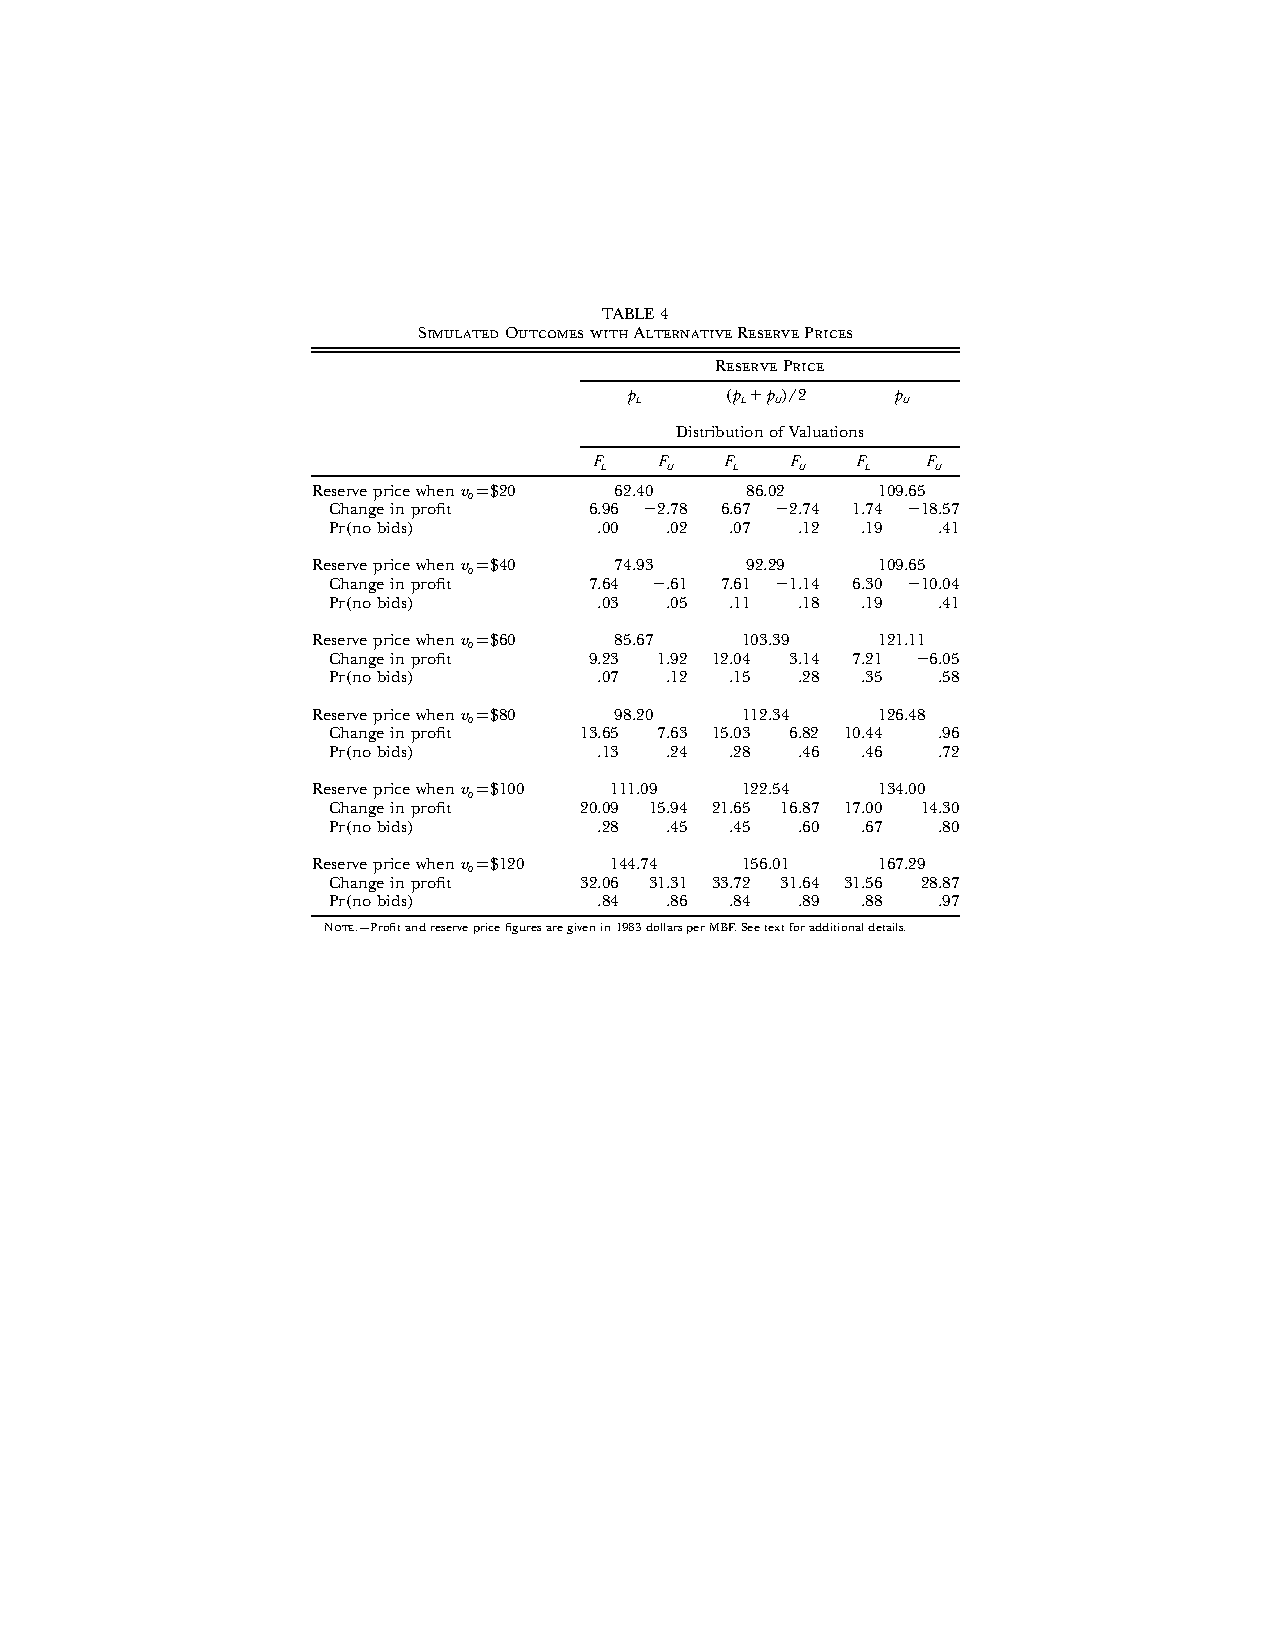
\includegraphics[scale=.7]{./resources/hailetamer4.pdf}
}

\begin{frame}{Moment Equalities}
We are already familiar with the idea of  \alert{moment equalities} of the form: $E[g(z_i,\theta)] = 0$:
\begin{itemize}
\item We can estimate them by forming $G_n(\theta)= \frac{1}{N} g_i(z_i,\theta)$  which is a $q \times 1$ vector.
\item Form the objective function $Q(\theta) = G_n(\theta)' * W * G_n(\theta)$ where $W$ is the $q \times q$ weighting-matrix.
\item Find $\hat{\theta}_{GMM} = \arg \max_{\theta} Q(\theta)$ where $\theta$ is $k \times 1$.
\item There is often a discussion about \alert{over} or \alert{under} or \alert{just} identification depending on whether $k > q$ or $k < q$ or $k=q$.
\begin{itemize}
\item When we are \alert{overidentified}: Often $Q(\hat{\theta}_{GMM}) > 0$ even if $E[g(z_i,\theta_0)]=0$ at the true population value $\theta_0$.
\item If we are \alert{underidentified} then $Q(\hat{\theta}_{GMM}) = 0$ at multiple values of $\theta$.
\end{itemize}
\end{itemize}
\end{frame}


\begin{frame}{Moment Inequalities: Chernozhukov, Hong, and Tamer (2007)}
Suppose we could make such a strong assumption, suppose instead that we were willing to assume $E[g(z_i,\theta)] \geq 0$.
\begin{itemize}
\item Instead of a single $\hat{\theta}$ we want to characterize a set $\Theta_I \subset \Theta$ that satisfies the moment inequality restrictions.
\item We can define $[x]_{+}$ to be the \alert{non-negative portion of x}: $x_j=\max\{x_j,0\}$.
\item We can define $[x]_{-}$ to be the \alert{non-positive portion of x}: $x_j=\min\{x_j,0\}$.
\item Now we can define the objective function: $Q(\theta) = E[g(z_i,\theta)]_{-}' \cdot W \cdot E[g(z_i,\theta)]_{-}$.
\item Or in finite sample $Q(\theta) = G_n(\theta)_{-}' * W * G_n(\theta)_{-}$
\item We want to find a $\theta$ to minimize $Q(\theta)$ but we only care about moment conditions that are violated from below (not from above).
\end{itemize}
\end{frame}

\begin{frame}{Moment Inequalities: CHT (2007)}
What is identified?
\begin{itemize}
\item Asymptotically we have that  $Q(\theta) = E[g(z_i,\theta)]_{-}' \cdot W \cdot E[g(z_i,\theta)]_{-}  = 0$.
\item What is identified is a \alert{set}. We might be tempted to define $\Theta_I = \{ \theta \in \Theta : Q(\theta) = 0\}$ and treat that as the \alert{identified set}.
\item What if we did that for the usual moment equality case (such as overidentified GMM)?
\begin{itemize}
\item Remember it can be that: $Q(\hat{\theta}_{GMM}) > 0$
\item Defining $\Theta_I = \{ \theta \in \Theta : Q(\theta) = 0\}$ might be a problem in finite sample.
\end{itemize}
\item Instead let $\Theta_I = \{ \theta \in \Theta : Q(\theta) = a_N\}$ where $a_N$ is some small positive number that gets smaller as $N$ gets larger.
\begin{itemize}
\item Most of the time $a_n = c / n$ (but you can cook up problems where this is not true!).
\end{itemize}
\end{itemize}
\end{frame}


\begin{frame}{Moment Inequalities: Inference}
Inference can be somewhat complicated.  We are now trying to construct a \alert{confidence set} rather than a \alert{confidence interval}
\begin{enumerate}
\item Should the confidence set contain each element of the identified set with a fixed probability (95\%)?
\item Should the confidence set the entire identified set some probability (95\%)?
\end{enumerate}
Most people work on (1).
\end{frame}


\begin{frame}{Moment Inequalities: Inference}
\begin{itemize}
\item Many estimated confidence sets tend to be \alert{conservative} that is they tend to be larger than they need to be.
\item For example, for each element of $\theta$ we could construct $[\theta_k^{LB},\theta_k^{UB}]$, but this assumes that the confidence set is a \alert{hyperrectangle} but it might be some ellipse wholly within that hyperrectangle.
\item Often we have some parameters that are \alert{point identified} while one one or two parameters are \alert{partially identified} within the same model.
\begin{itemize}
\item e.g.: We might know the determinants of the variable profits, but we might only be able to recover bounds on fixed costs or entry costs.
\end{itemize}
\end{itemize}
\end{frame}

\begin{frame}{Moment Inequalities: Inference}
There is a big (and fast growing) literature on how to construct confidence sets:
\begin{itemize}
\item Imbens and Manski (2004)
\item Romano and Shaikh (multiple papers)
\item Andrews and Soares, Andrews Berry Jia (2004).
\item Pakes, Porter, Ho, and Ishii (2015)
\end{itemize}
\end{frame}

\begin{frame}[fragile]{Example: $2 \times 2$ Entry Game}
\begin{center}
\begin{tabular}{cc|c|c|}
  & \multicolumn{1}{c}{} & \multicolumn{2}{c}{BK} \\
  & \multicolumn{1}{c}{} & \multicolumn{1}{c}{IN}  & \multicolumn{1}{c}{OUT}   \\\cline{3-4}
            & IN & $(\alpha_m + \delta_b + \epsilon_m, \alpha_b + \delta_m + \epsilon_b)$ & $(\alpha_m  + \epsilon_m, 0)$ \\ \cline{3-4}
McD  & OUT  & $(0, \alpha_b + \epsilon_b)$  & $(0,0)$  \\  \cline{3-4}
\end{tabular}
\end{center}
\begin{itemize}
\item Two players: Burger King and McDonald's.
\item Each player can play $(IN,OUT)$.
\item In market $i$ we can write the profits of $j$ as $\pi_{ij} = \alpha_{j} + \delta_{k} \cdot d_{ik} + X_i \beta+ \epsilon_{ij}$.
\item $d_{ij}=1$ if IN, $d_{ij}=0$ if OUT.
\item Competitive effect $\delta_k < 0$.
\item Firms observe everything (including $\epsilon$)
\end{itemize}
\end{frame}


\begin{frame}[fragile]{Example: $2 \times 2$ Entry Game}
Ignore covariates $\beta X_i$, suppose we have lots of data from independent plays of the game.
\begin{itemize}
\item $d_{ij} =1[\pi_{ij} \geq 0]$ (Firms enter when profits are positive).
\item Econometrician only observes entry status: $d_{ij} =1[\pi_{ij} \geq 0]$ for ${B,M}$.
\item Can we recover $\theta=[\delta_b,\delta_m,\alpha_a,\alpha_m]$? 
\item What if we assume that $\epsilon_{ij} \sim N(0,1)$ and is IID?
\end{itemize}
\end{frame}

\begin{frame}[fragile]{Example: $2 \times 2$ Entry Game}
What if:
\begin{eqnarray*}
-\alpha_B < \epsilon_B \leq -\alpha_B - \delta_M\\
-\alpha_M < \epsilon_M \leq -\alpha_M - \delta_B
\end{eqnarray*}
\begin{itemize}
\item Then $(d_b,d_m) = (1,0)$ and $(d_b,d_m) = (0,1)$ both satisfy the profit conditions!
\item This shouldn't be too surprising: the original game has \alert{multiple equilibria}.
\item We don't observe the \alert{selection rule} which determines behind the scenes which equilibria gets played.
\item Even if we knew the form of the errors $(\epsilon_b,\epsilon_m)$ we still can't map the data to a likelihood.
\item You cannot write $Pr((d_b,d_m) = (1,0))$ as a function of parameters!
\item We can make assumptions on the selection rule (Berry 1992) such as ``more profitable player moves first''.
\end{itemize}
\end{frame}

\frame{\frametitle{Entry Game}
\centering
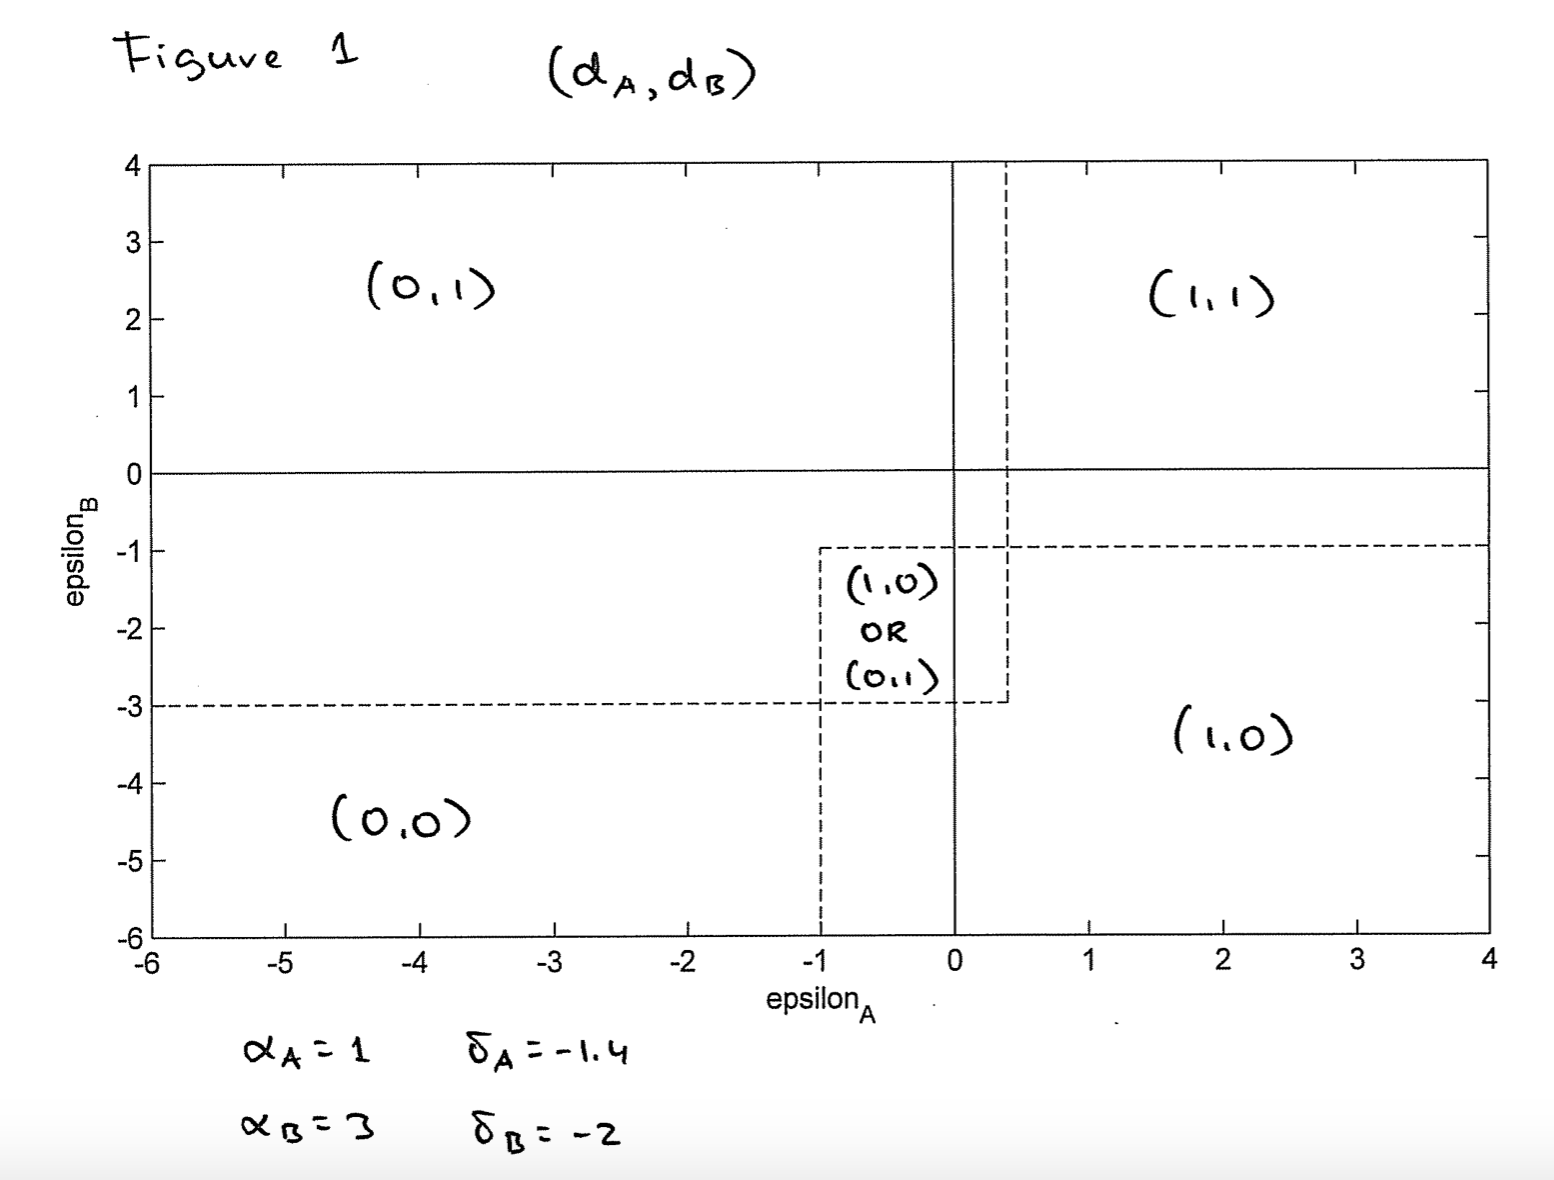
\includegraphics[width=4in]{./resources/entry1.png}
}


\begin{frame}[fragile]{Deriving Bounds}
\begin{eqnarray*}
H_{L,01}(\theta) \leq Pr ((d_{i,b}, d_{i,m}) = (0, 1)) \leq  H_{U,01}(\theta).
\end{eqnarray*}
Where
\begin{eqnarray*}
H_{L,01}(\theta) &=&Pr(\epsilon_{b} < -\alpha_b, -\alpha_m < \epsilon_m) +\\
&& Pr( -\alpha_b \leq \epsilon_{b} < -\alpha_b - \delta_b, -\alpha_m - \delta_m < \epsilon_m)
\end{eqnarray*}
and
\begin{eqnarray*}
H_{U,01}(\theta) &=&Pr(\epsilon_{b} < -\alpha_b, \alpha_m < \epsilon_m) +\\
&& Pr( -\alpha_b \leq \epsilon_{b} < -\alpha_b - \delta_b, -\alpha_m - \delta_m < \epsilon_m) +\\
&& Pr( -\alpha_b \leq \epsilon_{b} < -\alpha_b - \delta_b, -\alpha_m < \epsilon_m < -\alpha_m - \delta_m) 
\end{eqnarray*}
\end{frame}

\frame{\frametitle{Entry Game}
\centering
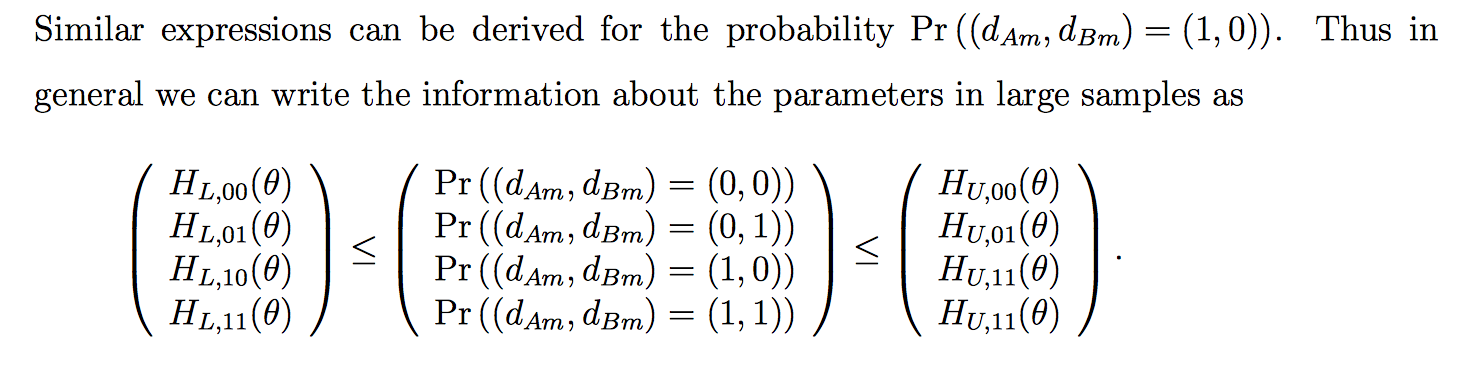
\includegraphics[width=4.5in]{./resources/entry3.png}\\
Note: For $d=(1,1)$ and $d=(0,0)$ the upper and lower bounds coincide.
}


\frame{\frametitle{Generalized Inequality Restrictions}
\centering
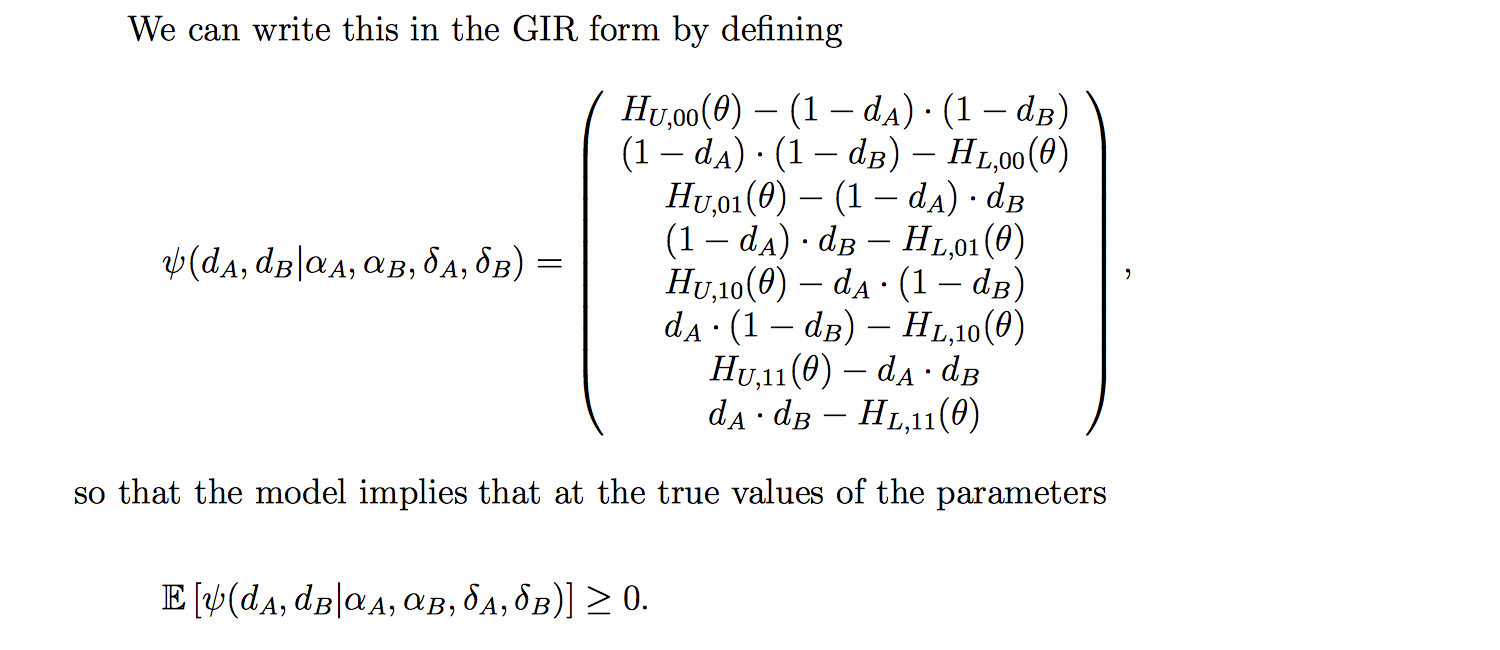
\includegraphics[width=5in]{./resources/entry2.png}
}

\frame{\frametitle{Generalized Inequality Restrictions}
\centering
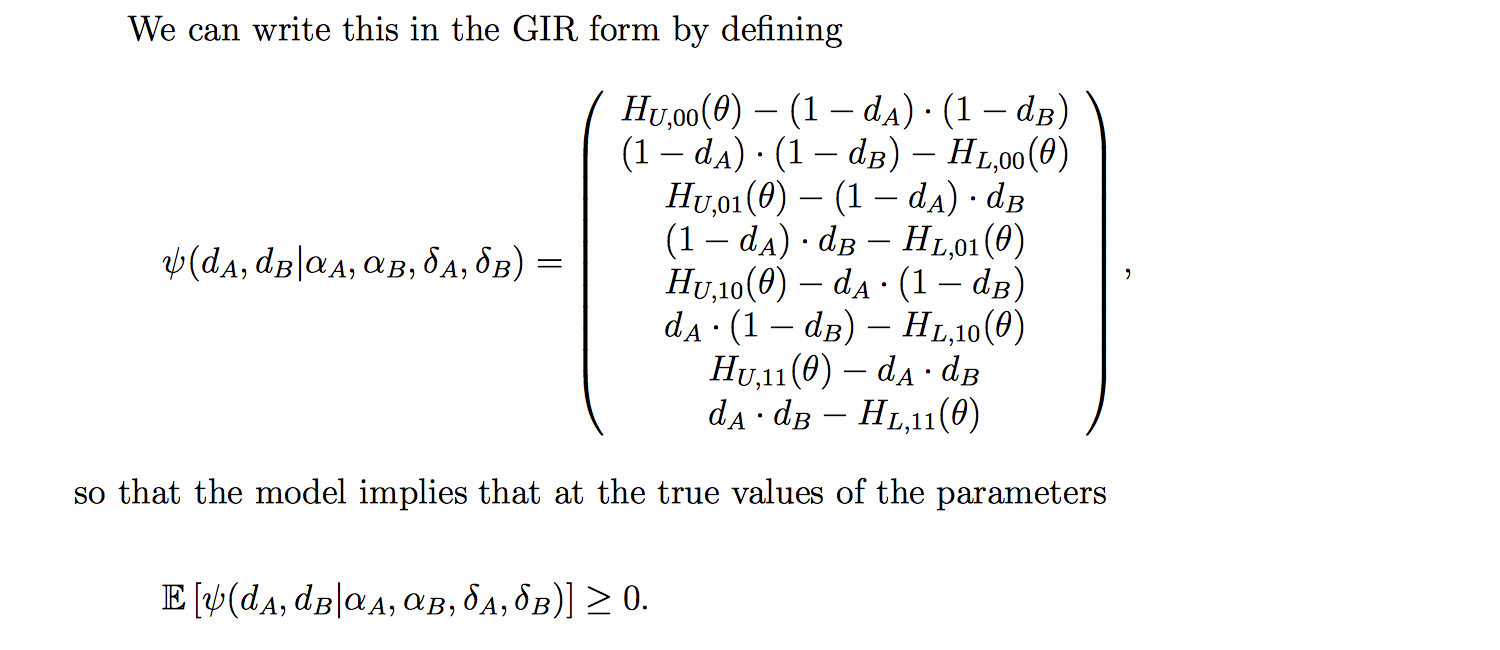
\includegraphics[width=5in]{./resources/entry2.png}
}



\begin{frame}[fragile]{Homework}
You can actually estimate this without too much difficulty ...
\end{frame}



%\setbeamertemplate{background canvas}{} 
%\includepdf[pages=1-4]{hailetamerall.pdf}



\end{document}
